\chapter{Future Work}
\label{sec:future}
In this section, we give an overview of possible areas of future work. We also point out deficiencies of \msname that we want to address in future versions.

\section{Classes as Instance-side Members}
\label{sec:future_inst_side}
Java and Newspeak support nested classes as instance-side members (non-static member classes). Earlier versions \msname included support for instance-side nested classes, but this caused difficulties in the implementation. 

\begin{itemize}
	\item \emph{Method lookup:} Classes can now be enclosed in instances instead of classes. We are not sure whether a message send to \texttt{enclosing}, \texttt{outer}, or \texttt{scope} should also lookup methods on the class side whenever a message was not understood on the instance side. It would certainly be good style to nest classes that do not need access to instance-specific state as class-side members. These classes should then be accessible within an instance using an implicit receiver send or the \texttt{scope} keyword.
	\item \emph{\texttt{outer}/\texttt{enclosing} cannot be early bound:} These keywords might have to start their lookup in an instance. Therefore, they cannot be bound as literals, which are stored in methods and, therefore, shared among all instances.
	\item \emph{Possible memory issues:} In contrast to Java, \msname would generate a new class every time an instance-side member class is accessed. This could lead to memory and performance issues.
\end{itemize}

In addition to these difficulties, we are currently unclear about what the exact benefits of instance-side nested classes are. They can be used to build mixins, but we achieve the same functionality with parameterized classes (see Section~\ref{sec:rel_mixins1}). In Java, non-static member classes are used to implement interface adapters that need access to the enclosing instance~\cite{Bloch:2008:EJ:1377533} (see Section~\ref{sec:rel_ns_pkg_cls_nesting}). This is, however, the only pattern for non-static member classes we could find in literature, and the same functionality can be achieved by implementing the adapter as a class-side nested class with an instance variable holding a reference to the adaptee.

As a consequence, we removed support for instance-side nested classes, but we might add it again at a later point of time, if it needed.

\section{Bytecode Transformation}
Whenever a nested class specification is instantiated in \msname, all methods in the specification are complied in the target class. When using parameterized classes, this process happens multiple times, once for every target class. However, the bytecode is almost the same for every target class and differs only for reads/writes to instance variables (see Section~\ref{sec:impl_ch_inst_cl_vars}). In addition, \texttt{enclosing} and \texttt{outer} must be bound to different literals.

This process could be optimized by caching compiled methods and replacing affected bytecodes and literals during instantiation. For example, instead of recompiling the entire method, all references to instance variables could be replaced with bytecodes with the correct indices in a linear pass through the compiled method.

In Newspeak, slots (instance variables) cannot be accessed directly. They are always accessed through automatically-generated accessor methods. Therefore, all references to slots are message sends. Consequently, the bytecode of a method for two different instantiations is always the same.

\section{Squeak Integration}
As of now, the integration of \msname in Squeak is still limited. For example, the new class browser does not have any refactoring tools yet. Furthermore, all Squeak classes should be migrated to classes in \msname, eventually, making \texttt{Repository} (a separate \texttt{globals} dictionary for \msname) obsolete. As described in Section~\ref{sec:impl_module_rep}, a single top-level class \texttt{Smalltalk} should contain all modules and Squeak base classes. Restructuring Squeak base classes in a hierarchical way will probably be the biggest and most tedious task. 

The Newspeak class organization might be a good starting point. Black et al. described how traits can be used to modularize Smalltalk collection classes~\cite{Black:2003:ATS:949305.949311}, which might be another good starting point for restructuring these classes.

\section{Extension Methods}
\label{sec:future_ext_meth}
In Smalltalk, an extension method is a method that extends an already existing class in another package. Additional methods can be defined on the instance side and and on the class side. Adding new instance/class variables or removing methods is not supported. In \msname, extension methods can be written by defining a class extension: a nested class with a class generator method that returns an already existing class.

Extension methods in Smalltalk and in \msname are controversial because they do not have proper conflict handling. If an extension method is defined and the target class has already a method with the same name, the original method is replaced, possibly breaking other code. Extension methods can be used to add new functionality to existing classes required by libraries (e.g., methods for the visitor design pattern). If two libraries add extension methods with the same name, the second extension always wins. In addition, removing an extension method does not restore the previous state: the original method has to be restored manually by the programmer.

Smalltalk extension methods break modularity. It is not possible to compose two modules providing colliding extension methods, because there is currently no way to resolve method conflicts without changing the source code of at least one of the modules. Furthermore, modules providing extension methods are not easily replacable, because the original state is not restored once a module is removed from the system.

Other programming languages (e.g., Ruby) have a concept similar to extension methods in Smalltalk. A variety of alternatives to extension methods have been proposed. In the rest of this chapter, we give a brief overview of some of them. Future versions of \msname might incorporate one of these alternatives.

\paragraph{Classboxes}
A classbox is a container of classes and methods. Classes can either be defined or imported into a classbox (from another classbox). Within a classbox, additional methods can be added or replaced on imported classes (\emph{local rebinding}). Code executed in the context of certain classbox has a modified method lookup: the system tries to lookup methods defined in the classbox first, and then proceeds with the ordinary method lookup (receiver class and superclass hierarchy)~\cite{bergel:inria-00533446}.

A classbox effectively acts as a sort of sandbox. Every classbox can define its own extensions methods for imported classes. Duplicate extension methods are not a problem as long as they are defined in different classboxes. 

Implementations of classboxes exist for Squeak~\cite{bergel:inria-00533446} and Java. Classbox/J is a Java implementation which does not only allow redefining fields and methods but also member classes (nested/inner classes)~\cite{Bergel:2005:CCS:1094811.1094826}.

\paragraph{Ruby Refinements}
In Ruby, all classes and modules are open for extensions. At any position in the program, existing classes can be modified, possibly breaking other code. Refinements are a way to confine class/module extensions to certain classes. A refinement can be defined as part of a module. Whenever the module is included, the refinement is active for code written in the including class~\cite{Carlson:2015:RC:1212915}. Other code is not affected.

\paragraph{Context-oriented Programming}
Context-oriented programming (COP) is a mechanism to modularize heterogeneous crosscutting concerns~\cite{Hirschfeld08context-orientedprogramming}. In layer-based context oriented programming, crosscutting concerns are grouped in layers. A layer is a set of partial method definitions (possibly from different classes). Every partial method definition belongs to exactly one base method. Whenever a layer is active, the system executes the partial methods defined in the layer instead of the corresponding base methods. Multiple layers can be active at the same time, effectively building a layer composition stack. A partial method can contain a \texttt{proceed} statement, which will call the next partial method, i.e., the partial method defined in the next layer on the layer composition stack. If there is no next layer defining a partial method for the corresponding base method, the system will call the base method.

Every module could group its extension methods in a separate layer, activate that layer whenever code from the module is run, and deactivate the layer afterwards. Most COP implementations support scoped layer activation~\cite{Appeltauer:2009:CCP:1562112.1562118}, which essentially activates a layer, then runs a method or function/block closure, and then deactivates the layer again.

With context-oriented programming, duplicate extension methods are no longer a problem, as long as they are contained in different layers as partial method definitions.

%\paragraph{Worlds}
%better way is needed (e.g., class boxes, refinements, COP, world (paper viewpoints), monkey patching). return already existing class in generator method

\section{Extending Inherited Nested Classes without Subclassing}
The way inherited nested classes can be extended without subclassing has two deficiencies. Firstly, there is currently no notation to add new instance variables to the extended class, because the subclass statement is part of the corresponding method in the superclass. Secondly, nested classes of already extended classes cannot be further extended, because a \texttt{super} call would not call the original class accessor method. Instead, the method lookup would start in the superclass of extended class (which is the same class as the not yet extended class).

It is still unclear, if extending inherited nested classes without subclassing should be forbidden in favor of the variant \emph{with subclassing}. Other programming languages like Jx do this by default~\cite{Nystrom:2004:SEV:1028976.1028986}. Extending inherited nested classes with subclassing would solve the problems described above and is already possible. However, forbidding \emph{extending without subclassing} is difficult without restricting the ability to write extension methods, which is technically a very similar concept.

\section{Dependency Management}
Nested classes in \msname can be used to store modules in different versions. There is at the moment no convenient way to share modules with other developers, except for exporting the module and importing it again. Future versions of \msname might have a central remote repository from which modules are automatically downloaded (similar to a Maven repository) if a module is referenced that is available in the image. The corresponding functionality could be part of a \texttt{doesNotUnderstand:} handler in \texttt{Repository}, which is the data structure holding references to all modules installed in the image.

There are also ideas for a better integration of the underlying source code management system (e.g., git) in \msname. If \msname is aware of commits, it can not only be used to run applications in certain versions, but also to run applications at a certain commit. Whether the source code management system should be completely reimplemented in \msname or be external and under control of \msname is still open to discussion.

\section{Language-supported Version Control}
In \msname, different versions of the same module are represented as different nested classes. The same mechanism could be used to integrate revision-based version control systems in Squeak/Smalltalk~\cite{springerniephaus}. Every revision/commit would then be represented by a separate nested class. \msname would ensure that nested classes are created automatically based on the revisions in the underlying version control system. Version control operations (e.g., commits and merges) could be invoked by sending messages to a nested class representing a revision.

\begin{figure}[!htp]
	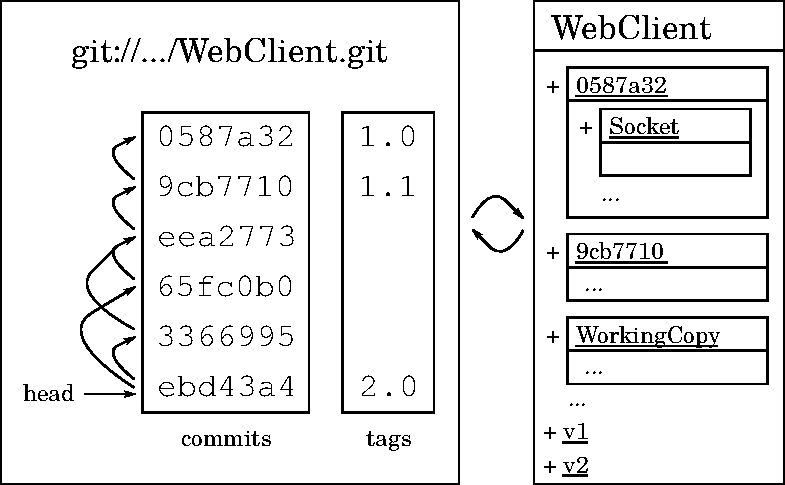
\includegraphics[width=0.75\textwidth]{matriona_concept.pdf}
	\centering
	\caption[Example: git-based version control with nested classes.]{Example: git-based version control with nested classes. \texttt{WebClient} is a module and every commit in the underlying version control system corresponds to an automatically-generated nested class in \msname.}
	\label{fig:fut_vers_control_git}
\end{figure}

Figure~\ref{fig:fut_vers_control_git} shows an example of a module named \texttt{WebClient}. The source code is stored in a git repository. Every commit in git corresponds to a nested class whose name is the SHA-1 hash of the commit. \msname takes care of the synchronization between the repository and the nested classes in the Squeak image. The programmer would always modify the source code in the class \texttt{WorkingCopy} and send a message like \texttt{commit:} to this class in order to perform a commit in the git repository. git tags could be used to provide a versioning scheme that is mirrored in the version control system.

This mechansim would allow the programmer to access any revision in the Squeak image without having to load the source code for a certain revision manually. Furthermore, multiple revisions of the same module could be run at the same time. Having version control in the Squeak image would also reduce the number of tools involved in the software development process and get rid of the conceptual break of leaving the image for committing to a git repository (see Section~\ref{sec:impl_scm_chap}).
% automatically download dependencies
% generate list of all dependencies